\documentclass{standalone}
\usepackage{tikz}
\begin{document}
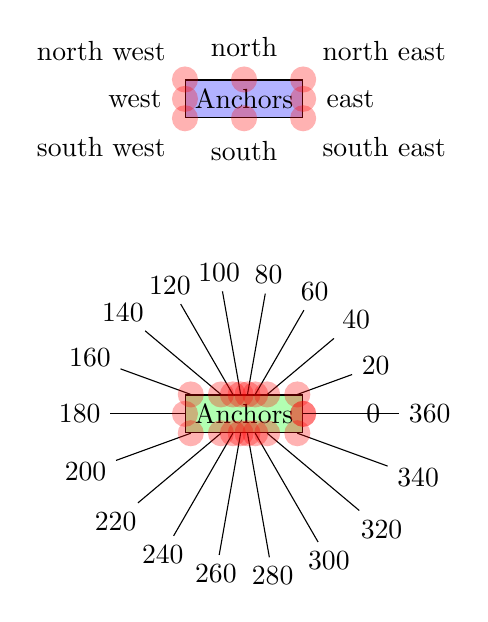
\begin{tikzpicture}[fill opacity=.3,text opacity=1]

\node[draw,fill=blue] (A) at (0,4) {Anchors};

\foreach \a in {north,east,south,west,
    north east,north west,south west,south east}{
    \node[fill=red,circle,label=\a:\a] at (A.\a) {};
}

\node[draw,fill=green] (B) at (0,0) {Anchors};

\foreach[count=\i] \a in {0,20,...,360}{
    \draw (B) -- +(\a:1.4+.03*\i) node[anchor=180+\a]{\a};
    \node[fill=red,circle] at (B.\a) {};
}

\end{tikzpicture}
\end{document}
